\chapter{Functions}
\label{sec:4}
In mathematics, a function is a binary relation over two sets that associates every element of the first set, to exactly one element of the second set.
If the function is called $f$, this relation is denoted by $y = f (x)$, where the element $x$ is the input of the function, and $y$ is the value of the function that is the output.
In mathematical language, pratyayas can be defined as functions, which	can be applied to various dhātus say $x$, to give the corresponding word as shown in Figure~\ref{fig:x}.
\begin{figure}[!h]
	\centering
	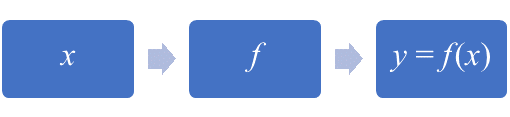
\includegraphics[width=1.0\textwidth]{function.png}
	\hspace{1mm}
	\caption{Function $f(x)$} 
	\label{fig:x}
\end{figure}

\section{Function p(x)}
The input dhātus are categorized as seṭ and aniṭ to determine whether an \texthindi{इ} is added before the addition of a pratyaya or not. This however, is different from the \texthindi{इ} that is added due to the addition of the \texthindi{णिच्} pratyaya. When the \texthindi{णिच्} pratyaya is added only \texthindi{इ} remains and the rest is removed. To differentiate between the two \texthindi{इ}s, only \texthindi{इ} is added when the addition is due to the input dhātu being seṭ, and when it is added due to the addition of the \texthindi{णिच्} pratyaya, it is written as \texthindi{इ(णिच्)} which should be read as \texthindi{इ} due to \texthindi{णिच्}. Note that this differentiation is required only when both types of \texthindi{इ} occur simulataneously in the same equation.  Thus \texthindi{इ(णिच्)} becomes a part of the prakṛti, whereas the \texthindi{इ} due to \texthindi{णिच्} pratyaya is a pratyaya. \\
The dhātus which have two or more vowels are called seṭ (with iṭ), and when a suffix is added to them an \texthindi{इ} comes. For dhātus which have one vowel, we need to see the instructions given in the Dhātupātha. They can either be seṭ or aniṭ depending upon the given instructions given. As it is a global function which is used in the definition of other pratyaya functions, it is important to define it here.\\
Define a function p(x) by, \\
\begin{equation}
	p(x)= \begin{cases}
		\text{\texthindi{इ}} & \text{if $x$ is \texthindi{ सेट्}}\\
		\phi&  \text{ if $x$ is \texthindi{ अनिट्}}\\
	\end{cases}
\end{equation}
\section{The $+$ operator}

\label{sec:operator}
The $+$ operator can be compared to Sandhi in grammar. It has been used extensively in the formulas. Some of the cases which might be observed in the various examples have been enumerated below.\\
For seṭ Dhātus:\\

\begin{center}
	\begin{tabular}{ p{4cm} p{4cm} p{4cm} }
		
		\texthindi{क्+इ=कि}&
		\texthindi{ख्+इ=खि}&
		\texthindi{ग्+इ=गि}\\
		\texthindi{घ्+इ=घि}&
		\texthindi{च्+इ=चि}&
		\texthindi{छ्+इ=छि}\\
		\texthindi{ज्+इ=जि}&
		\texthindi{ट्+इ=टि}&
		\texthindi{ठ्+इ=ठि}\\
		\texthindi{त्+इ=ति}&
		\texthindi{थ्+इ=थि}&
		\texthindi{द्+इ=दि}\\
		\texthindi{ध्+इ=धि}&
		\texthindi{प्+इ=पि}&
		\texthindi{ऊ+इ=वि}\\
		\texthindi{ए+इ=अयि}&
		\texthindi{ब्+इ=बि}&
		\texthindi{व्+इ=वि}\\
		\texthindi{भ+इ=भि}&
		\texthindi{फ्+इ=फि}&
		\texthindi{ण्+इ=णि}\\
		\texthindi{न्+इ=नि}&
		\texthindi{म्+इ=मि}&
		\texthindi{य्+इ=यि}\\
		\texthindi{ल्+इ=लि}&
		\texthindi{र्+इ=रि}&
		\texthindi{क्ष्+इ=क्षि}\\
		\texthindi{ष्+इ=षि}&
		\texthindi{स्+इ=सि}&
		\texthindi{ह्+इ=हि}\\
		\texthindi{श्+इ=शि}&
		\texthindi{झ्+इ=झि}&
		\texthindi{ञ्+इ=ञि}\\
		\texthindi{ङ्+इ=ङि}&
		\texthindi{ढ+इ=ढि}&
		\texthindi{ओ+इ=अवि}\\
		
	\end{tabular}
\end{center}


Similarly, for aniṭ dhātus:
\\
\begin{center}
	\begin{tabular}{ p{4cm} p{4cm} p{4cm}}
		\texthindi{क्+त=क्त}&
		\texthindi{ र्+त=र्त}&
		\texthindi{ द्+त=त्त}\\
		\texthindi{ ष्+त=ष्ट}&
		\texthindi{ च्+त=च्त}&
		\texthindi{ छ्+त=ष्ट}\\
		\texthindi{ ज्+त=क्त}&
		\texthindi{ ण्+त=न्त}&
		\texthindi{ त्+त=त्त}\\
		\texthindi{ ध्+त=ध्द}&
		\texthindi{ न्+त=न्त}&
		\texthindi{ प्+त=प्त}\\
		\texthindi{ भ्+त=ब्ध}&
		\texthindi{ म्+त=तं}&
		\texthindi{ श्+त=श्त}\\
		\texthindi{ स्+त=स्त}&
		\texthindi{ ह्+त= ण्ढ}&
		
	\end{tabular}
\end{center}

\section{Input Dhātus (x)}
The primary list of input dhātus are taken from Madhaviya Dhātuvṛtti which are enumerated in set $A$. Let $A$ be a set of all the dhātus after the Anubandha has been removed.\\

$A$ = [\texthindi{दा धा मा गा हा पा शा षा छा वा रा जा सा का या भा ला दरिद्रा स्था ज्या व्या क्षा ग्ला म्ला द्या श्रा द्रा ध्मा प्या श्या प्रा त्रा स्त्या घ्रा ध्रा म्ना ध्या स्ना प्सा ज्ञा ख्या ह्वा श्रि श्वि ज्रि स्मि जि कि हि रि पि धि इ सि शि चि मि चिरि जिरि प्री व्री ह्री भ्री क्षी व्ली प्ली क्री श्री री पी शी नी दी मी धी ली डी भी वी ई मी दीधी वेवी ऊर्णु कु ध्रु गु स्तु द्रु स्रु श्रु धु दु सु धु धू नु यु रु क्षु क्ष्णु स्नु उ गु कु घु ङु च्यु ज्यु प्रु प्लु रु ह्नु हु कु सु दु द्यु सु स्कु यु ब्रु नू धू मू सू पू दू लू नू क्नू धू सू भू स्वृ ध्वृ ह्वृ स्मृ स्पृ स्तृ हृ गृ घृ पृ दृ सृ ॠ जागृ धृ पृ दृ मृ धृ हृ भृ कृ वॄ भॄ मॄ पॄ स्तॄ कॄ शॄ दॄ तॄ जॄ झॄ गॄ नॄ ऋ(प्लुत) अक् शक् तक् चक् स्तक् कक् कख् बख् मख् नख् रख् लख् अग् लग् रग् सग् हग् ह्वग् ह्लग् स्तग् कग् घघ् सघ् दघ् वच् व्यच् खच् खम् पच् त्वच् सच् शच् मच् श्वच् कच् अज् यज् भज् त्यज् लज् जज् ध्रज् घ्वज् खज् गज् वज् व्रज् अट् घट् कट् वट् भट् णट् नट् पट् रट् लट् शट् सट् वट् जट् झट् भट् तट् खट् हट् पठ् मठ् रठ् शठ् वठ् कठ् हठ् अड् लड् कड् गड् अण् क्षण् फण् रण् मण् वण् भण् कण् क्वण् व्रण् भ्रण् ध्वण् श्रण् चण् शण् चण् रण् पण् अत् यत् चत् फत् क्वथ् पथ् मथ् व्यथ् प्रथ् श्रथ् श्लथ् क्लथ् क्रथ् अद् सद् शद् मद् बद् रद् नद् खद् वद् हद् पद् दद् स्वद् व्रद् श्खद् चद् बध् व्यध् रध् दध् वन् मन् तन् वन् जन् खन् सन् कन् स्वन् स्तन् ध्वन् धन् ध्रण् पन् हन् अन् स्वप् तप् वप् शप् क्रप् जप् चप् सप् रप् लप् त्रप् रफ् कब् रभ् लभ् जभ् यभ् नभ् गम् नम् यम् रम् भ्रम् शम् तम् दम् श्रम् शम् क्लम् क्षम् कम् क्रम् छम् झम् जम् जिम् चम् सम् स्तम् स्यम् वम् द्रम् अम् अय् दय् वय् पय् मय् चय् तय् नय् रय् वय् हय् त्वर् ज्वर् चर् त्सर् क्मर् क्षर् अल् फल् चल् जल् नल् पल् बल् सल् दल् शल् तल् ट्वल् स्थल् हल् ज्वल् ह्वल् ह्मल् स्खल् खल् गल् श्वल् मल् शल् वल् भल् कल् अव् मव् शव् अश् नश् मश् शश् वश् स्पश् चष् लष् छष् झष् मष् शष् जष् कष् खष् वष् भष् अस् उध्रस् ध्रस् घस् जस् तस् दस् मस् यस् वस् शस् सस् रस् लस् त्रस् स्नस् क्नस् ह्रस् व्लस् कस् घस् हस् प्रस् नस् ग्रस् ग्लस् वस् भ्यस् दह् वह् सह् नह् रह् मह् चह् ग्लह् ग्रह् अह् \\
	टिक् तिक् इख् लिख् तिग् स्तिघ् सिच् रिच् विच् निज् विज् तिज् इट् किट् खिट् शिट् सिट् चिट् बिट् विट् पिट् पिठ् क्षिण् कित् चित् श्वित् विथ् स्विद् मिद् क्षिद् मिद् स्विद् क्लिद् विद् भिद् क्षिद् विद् खिद् निद् मिद् सिध् विध् क्षिप् लिप् तिप् स्तिप् डिप् रिफ् तिम् स्तिम् इल् मिल् तिल् किल् चिल् विल् बिल् निल् हिल् मिल् शिल् सिल् ष्ठिव् क्षिव् सिव् दिव् स्रिव् दिश् लिश् रिश् विश् क्लिश् लिश् मिश् निश् पिश् इष् शिष् रिष् जिष् मिष् श्रिष् विष् ध्रिष् श्लिष् द्विष् विष् रिष् शिष् पिष् विष् त्विष् पिस् बिस् स्निह् दिह् लिह् मिह् प्लिह् \\
	कुक् उख् मुच् शुच् रुच् स्तुच् म्रुच् म्लुच् ग्रच् ग्लुच् शुच् कुच् उच् रुज् भुज् कुज् खुज् तुज् मुज् गुज् युज् भुज् स्फुट् रुट् लुट् घुट् कुट् पुट् मुट् त्रुट् तुट् चुट् छुट् घुट्  लुठ् रुठ् शुठ् उठ् मुड् प्रुड्हड् तुड् जुड् कुड् पुड् तुड् थुड् स्थुड् गुड् स्फुड् चुड् व्रुड् रुड् घुण् तुण् द्रुण् पुण् मुण् कुण् च्युत् श्चुत् श्च्युत् युत् जुत् द्युत् कुथ् पुथ् मुद् गुद् तुद् नुद् शुद् रुद् नुद् बुध् गुध् क्रुध् क्षुध् शुध् रुध् युध् अनुरुध् शुन् गुप् लुप् छुप् तुप् त्रुप् चुप् कुप् युप् रुप् लुप् तुफ् त्रुफ् गुफ् शुभ् स्तुभ् तुभ् क्षुभ् लुभ् क्षुभ् उभ् गुर् छुर् स्फुर् तुर् सुर् खुर् कुर् मुर् शुर् घुर् पुर् श्फुल् पुल् कुल् हुल् क्रुश् रुश् उष् शुष् तुष् दुष् पुष् व्युष् प्लुष् घुष् पुष् रुष् प्रुष् प्लुष् व्युष् मुष् कुष् जुष् बुस् मुस् कुस् तुस् श्नुस् दुह् तुह् सुह् रुह् ध्रुह् मुह् स्नुह् गुह् उह् \\
	वृक् ॠच् पृच् ॠज् धृज् गृज् वृज् मृज् सृज् भृज् कृड् भृड् मृड् पृड् ऋण् पृण् वृण् मृण् तृण् घृण् वृत् नृत् कृत् चृत् वृत् शृद् तृद् मृद् ऋध् गृध् वृध् शृध् मृध् कल्प् सृप् त्रृप् दृप् ऋफ् सृभ् दृभ् स्पृश् वृश् दृश् भृश् कृश् हृश् तृष् पृष् वृष् मृष् घृष हृष् धृष् कृष् ऋष् दृह् बृह् तृह् वृह् स्तृह् गृह् \\
	अन्क् तन्क् स्रन्क् शन्क् श्लन्क् शन्क् वन्क् मन्क् कन्क् श्वन्क् त्रन्क् शीक् टीक् तीक् द्रेक् ध्रेक् रेक् सेक् स्त्रेक् लोक् श्लोक् ढौक् त्रौक् ष्वष्क् वस्क् मस्क् फक्क् बुक्क् पुक्क् हिक्क् ओख् इन्ख् ईन्ख् उन्ख् वन्ख् मन्ख् रन्ख् नन्ख् लन्ख् राख् लाख् द्राख् ध्राख् शाख् श्लाख् अन्ग् इङ्ग रन्ग् लन्ग् वन्ग् मन्ग् तन्ग् शन्ग् श्लन्ग् रिन्ग् लिन्ग् थन्ग् युन्ग् जुन्ग् बुन्ग् वल्ग् अन्घ् मन्घ् रन्घ् लन्घ् वन्घ् मन्घ् शिन्घ् राघ् लाघ् द्राघ् श्लाघ् अञ्च् अर्च् लुञ्च् वञ्च् कुञ्च् चञ्च् तञ्च् त्वञ्च् म्रुञ्च् म्लुञ्च् ग्लुञ्च् तञ्च् कुञ्च् श्वन्च् शन्च् कन्च् कान्च् मुन्च् मन्च् पन्च् याच् लोच् वर्च् चर्च् व्रश्च् ऋच्छ आन्छ उन्छ् उञ्छ् उच्छ् प्रच्छ् लान्छ् वान्छ् हुर्च्छ् स्फूर्च्छ् मूर्च्छ् विच्छ् मिच्छ् युच्छ् लच्छ् ह्रीच्छ् म्लेच्छ् ऋन्ज् ईज् एज् उब्ज् अर्ज् अञ्ज् रञ्ज् भञ्ज् सञ्ज् गुन्ज् ध्रन्ज् धृन्ज् ध्वन्ज् खन्ज् लन्ज् लान्ज् जन्ज् तुन्ज् गन्ज् गृन्ज् मुन्ज् लाज् क्षीज् कूज् तेज् सर्ज् गर्ज् तर्ज् कर्ज् खर्ज् जर्ज् स्फूर्ज् मज्ज् क्षन्ज् निंज् शिंज् पिंज् स्वञ्ज् लज्ज् भ्रेज् भ्राज् राज् सज्ज् भ्रज्ज् झर्झ् उज्झ् अट्ट् घट्ट् वेष्ट् चेष्ट् गोष्ट् लोष्ट् रेट् रुन्ट् लुन्ट् म्लेट् शौट् यौट् एठ् अन्ठ् वन्ठ् मन्ठ् कन्ठ् मुन्ठ हेठ् कुन्ठ् लुन्ठ् शुन्ठ् रुन्ठ् कुन्ड् चुन्ड् गन्ड् मन्ड् वन्ड् भन्ड् चन्ड् शन्ड् तन्ड् पन्ड् कन्ड् खन्ड् हिन्ड् पिन्ड् हुन्ड् कुन्ड् मुन्ड् तुन्ड् बाड् द्राड् ध्राड् शाड् हेड् होड् क्रीड् व्रीड् हूड् म्रेड् हेड् होड् रोड् लोड् रौड् चुड्ड् कड्ड् अड्ड् ईड् ओण् पैण् शोण् श्रोण् श्लोण् घूर्ण् वेण् घिन्ण् घुन्ण् घृन्ण् धूर्ण् अन्त् संस्त् कुन्थ् पुन्थ् लुन्थ् मन्थ् ग्रन्थ् कुन्थ् श्रन्थ् ग्रन्थ् कत्थ् वेथ् नाथ् प्रोथ् अर्द् अन्द् इन्द् उन्द् उर्द् बुन्द् मेद् नेद् वन्द् भन्द् मन्द् स्पन्द् कन्द् क्रन्द् क्लन्द् श्विन्द् स्कुन्द् क्लिन्द् कूर्द् खूर्द् गूर्द् पर्द् स्वर्द् स्वाद् ह्राद् ह्लाद् सूद् स्यन्द् स्कन्द् नर्द् गर्द् तर्द् कर्द् खर्द् त्रन्द् कन्द् क्रन्द् क्लन्द् चन्द् नन्द् बिन्द् निन्द् क्लिन्द् खाद् इन्ध् एध् शुन्ध् बन्ध् राघ् साध् मेध् नाध् बाध् गाध् स्पर्ध् मान् दान् शान् धूप् तुम्प् त्रुम्प् पर्प् जल्प् पुष्प् कन्प् दीप् तेप् स्तेप् ग्लेप् वेप् केप् गेप् ग्लेप् मेप् रेप् लेप् आप् ॠम्फ् रन्फ् तुम्फ् त्रुम्फ् तृम्फ् दृम्फ् तुम्फ् गुम्फ् अर्ब् अन्ब् क्लीब् क्षीब् रन्ब् लन्ब् कुन्ब् लुन्ब् तुन्ब् चुन्ब् पर्ब् लर्ब् बर्ब् भर्ब् कर्ब् खर्ब् गर्ब् शर्ब् सर्ब् चर्ब् उम्भ् दम्भ् शुम्भ् सृम्भ् श्रम्भ् स्रम्भ् स्तन्भ् स्कन्भ् जृन्भ् शीभ् चीभ् रेभ् शल्भ् वल्भ् गल्भ् भाम् हम्म् स्तीम् मीम् ऊय् ईर्क्ष्य् ईर्ष्य् मव्य् शुच्य् हर्य् सूर्क्ष्य् चाय् ताय् क्ष्माय् स्फाय् पूय् क्नूय् प्याय् ईर् अभ्र् वभ्र् मभ्र् खोर् धोर् पूर् तूर् धूर् गूर् घूर् जूर् शूर् चूर् वेल् चेल् केल् खेल् क्ष्वेल् पेल् फेल् शेल् खोल् मील् श्मील् स्मील् क्ष्मील् पील् नील् शील् कील् कूल् शूल् तूल् पूल् मूल् खल्ल् चिल्ल् चुल्ल् फुल्ल् वेल्ल् वल्ल् कल्ल् मल्ल् भल्ल् इन्व् ऊर्व् अर्व् रन्व् धन्व् पिन्व् मिन्व् निन्व् हिन्व् दिन्व् धिन्व् जिन्व् रिन्व् कृण्व् पीव् मीव् तीव् नीव् जीव् क्षेव् मूर्व् तूर्व् थूर्व् दूर्व् धूर्व् गूर्व् पर्व् सर्व् मर्व् चर्व् भर्व् कर्व् खर्व् गर्व् शर्व् पूर्व् चीव् धाव् तेव् देव् सेव् गेव् ग्लेव् पेव् मेव् म्लेव् रेव् ईश् क्लेश् काश् वाश् भ्राश् भ्लाश् दंश् भ्रंश् दाश् ईष् ऊष् ईष् एष् चूष् तूष् पूष् मूष् लूष् रूष् शूष् यूष् जूष् भूष् घुन्ष् वर्ष् भाष् गेष् ग्लेष् पेष् जेष् नेष् प्रेष् रेष् हेष् ह्रेष् भेष् भ्रेष् भ्लेष् ईक्ष् उक्ष् अक्ष् तक्ष् रक्ष् त्रक्ष् स्त्रक्ष् नक्ष् वक्ष् जक्ष् निक्ष् मृक्ष् सूर्क्ष् कान्क्ष् वान्क्ष् मान्क्ष् द्रान्क्ष् ध्रान्क्ष् ध्वान्क्ष् भ्रक्ष् भ्लक्ष् त्वक्ष् दक्ष् ध्रिक्ष् शिक्ष् भिक्ष् दीक्ष् धुक्ष् वृक्ष् चक्ष् आस् स्रंस् ध्वंस् भ्रंस् आशन्स् कंस् निंस् कास् भास् नास् रास् आशास् दास् पेस् शास् चकास् हिंस् शंस् ईह् ऊह् अन्ह् अर्ह् तृंह् रन्ह् दृन्ह् बृन्ह् बन्ह् मन्ह् गर्ह् बर्ह् वर्ह् बल्ह् गल्ह् वल्ह् बाह् द्राह् वेह् जेह् गाह् माह् \\
	चुरादिगण- चि जि ज्रि प्री ली मी भू धू वृ पॄ जॄ वच् पट् घट् नट् तड् पत् तड् पत् श्रथ् नद् छद् वद् आसद् स्वद् तन् तप् दल् नल् जस् उध्रस् ग्रस् सह् रिच् दिव् शिष् रुज् युज् पुट् लुट् रुट् पुथ् गुप् कुप् जुष् पुष् घुष् पृच् वृज् मृज् वृत् छृद् शृध् वृध् तृप् दृभ् मृष् धृष् वल्क विष्क लोक् तर्क् शीक् चीक् टन्क् दुःख मार्ग् लिन्ग् लन्घ् रन्घ् लन्घ् लोच् पन्च् वन्च् अञ्च् अर्च् विच्छ् मिन्ज् पिन्ज् लुन्ज् भन्ज् तुन्ज् छन्ज् लन्ज् अन्ज् वन्ट् घन्ट् पुन्ट् चुन्ट् शुन्ठ् कन्ठ् दण्ड स्फुन्ड् लन्ड् खन्ड् कन्ड् कुन्ड् गुन्ड् खुन्ड् मन्ड् भन्ड् पन्ड् पिन्ड् लन्ड् वर्ण पर्ण चिन्त् पन्थ् ग्रन्थ् श्रन्थ् तुत्थ मिन्द् छन्द् अर्द् शुन्ध् मान् आप् धूप् चम्प् क्षम्प् चुम्ब् कुम्ब् लुम्ब् तुम्ब् जम्भ् कत्र चित्र मूत्र ईर् पूर् चीव् गर्व छिद्र मिश्र दंश् कुंश् भृंश् रुंश् रूक्ष त्रंस् पिंस् कुंस् दंस् रुंस् जंस् तंस् पंस् हिंस् दंस् अंह् बृंह् रंह् मंह् अर्ह् गर्ह् बर्ह् बल्ह् ज्ञा च्यु भू यु गृ घृ रक् लग् रच लज व्रज् गज् भज् नट् चट् घट् पट वट शठ श्वठ शठ् श्वठ् शठ् तड् खड् लड् श्रण् कण् gaṇa व्रण यत् श्रय् प्रथ् श्रथ कथ गद छद पद मद् बध् ध्वन स्तन ज्ञप् ह्लप् डप् अम् शम् स्यम् यम् व्यय वर स्वर चर् क्षल् तल् जल् कल् कल बल् चल् लल् गल् भल् पश् स्पश् लस् त्रस् नस् रस वस रह् मह रह चह तिज् स्मिट् चित् विद् डिप् क्षिप विल् बिल् तिल् इल् श्लिष् पिस् स्नेह् सुख मुच् चुट् मुट् स्फुट् त्रुट् पुट् शुठ् जुड् कुण गुण चुद् मुद् स्तुप् चुर् तुल् दुल् पुल् चुल् रुष् कुह मृग पृथ् कल्प् कृप वृष् गृह स्पृह बुक्क् नक्क् धक्क् चक्क् चुक्क् श्वल्क् वल्क् शुल्क् अर्क् विष्क् निष्क् अङ्क अङ्ग धेक सूच चर्च् मर्च् म्लेच्छ् पिच्छ् पूज् मार्ज् अर्ज् तर्ज् ऊर्ज् भाज सभाज कीट् घट्ट् खट्ट् सट्ट् स्फिट्ट् कुट्ट् पुट्ट् चुट्ट् अट्ट् सुट्ट् कूट् कूट खेट क्षोट लुण्ठ् ईड् पीड् चूर्ण् वर्ण् कूण् तूण् भ्रूण् क्रूण मुस्त् पुस्त् बुस्त् श्वर्त् कॄत् बस्त् वात संकेत केत अर्थ गूर्द् शब्द् सूद् आक्रन्द् छर्द् छेद अन्ध्र गन्ध् वर्ध् मान् ऊन स्तेन रूप शूर्प् सम्ब् शम्ब् शुल्ब् लाभ भाम साम ग्राम सङ्ग्राम गोम स्तोम कुस्म् सार पार तीर सूत्र कुमार श्वभ्र् गूर् शूर वीर सत्र यन्त्र् तन्त्र् मन्त्र् कुन्द्र् पूल् मूल् पाल् स्थूल शील वेल पल्यूल सान्त्व् भूष् लूष् गवेष लक्ष् पक्ष् यक्ष् भक्ष् म्रक्ष् पुंस् धूस् ब्रूस् भर्त्स् कुत्स् वास निवास अंस बर्ह् अर्ह् सुख दुःख लिट लाट गद्गद अगद वेद मगध इषुध कुषुभ तरण चरण वरण चुरण तुरण भुरण सपर अरर अम्बर संवर लेखा रेखा लेला मेधा एला केला खेला इला मही हृणी मन्तु वल्गु कण्डू असू असु इर् इरज् भिषज् भिष्णज् लेट् लोट् इरस् उषस् तन्तस् पम्पस् द्रवस् तिरस् उरस् पयस् संभूयस्}]
\\
These primary dhātus are 1943 in total. However, the input dhātus are not limited to these dhātus in set $A$. We can also derive a new dhātu by adding a san pratyaya to the dhātus of set $A$. By ‘3.1.32 \texthindi{सनाद्यन्ताः धातवः}’ the derived dhātus also becomes a dhātu as it says that whenever we add a \texthindi{सनादि} pratyaya to a Dhātu, it again becomes a Dhātu. \\

There are several ways of deriving Dhātus:\\
By adding a suffix to any Dhātu (enlisted in set $B$)\\
Derving Dhātus from nouns i.e. nāmdhātu $(j(x)) $(enlisted in set $C$)\\

List of \texthindi{सनादि} pratyayas in Aṣhṭādhyāyī with their respective sūtra numbers:\\
\begin{itemize}
	\item \texthindi{3.1.5 सन्}
	\item \texthindi{3.1.8 क्यच्}
	\item \texthindi{3.1.9 काम्यच्}
	\item \texthindi{3.1.11 क्यङ्}
	\item \texthindi{3.1.13 क्यष्}
	\item \texthindi{3.1.20 णिङ्}
	\item \texthindi{3.1.21 णिच्}
	\item \texthindi{3.1.22 यङ्}
	\item \texthindi{3.1.27 यक्}
	\item \texthindi{3.1.28 आय्}
	\item \texthindi{3.1.29 ईयङ्}
\end{itemize}
$B$ is a set of all the derived dhātus that are derived by adding san pratyayas to the set $A$. \\
$C$ is a set of nāmdhātus\\
\begin{equation}
	x \epsilon (A \cup B \cup C)
\end{equation}

